\documentclass[journal]{IEEEtran}

\usepackage{tikz}
\usetikzlibrary{shapes.multipart}  
\usepackage{pgfplots}


\pgfplotsset{
    box plot/.style={
        /pgfplots/.cd,
        black,
        only marks,
        mark=-,
        mark size=0.2em,
        /pgfplots/error bars/.cd,
        y dir=plus,
        y explicit,
    },
    box plot box/.style={
        /pgfplots/error bars/draw error bar/.code 2 args={%
            \draw  ##1 -- ++(0.2em,0pt) |- ##2 -- ++(-0.2em,0pt) |- ##1 -- cycle;
        },
        /pgfplots/table/.cd,
        y index=2,
        y error expr={\thisrowno{3}-\thisrowno{2}},
        /pgfplots/box plot
    },
    box plot top whisker/.style={
        /pgfplots/error bars/draw error bar/.code 2 args={%
            \pgfkeysgetvalue{/pgfplots/error bars/error mark}%
            {\pgfplotserrorbarsmark}%
            \pgfkeysgetvalue{/pgfplots/error bars/error mark options}%
            {\pgfplotserrorbarsmarkopts}%
            \path ##1 -- ##2;
        },
        /pgfplots/table/.cd,
        y index=4,
        y error expr={\thisrowno{2}-\thisrowno{4}},
        /pgfplots/box plot,
    },
    box plot bottom whisker/.style={
        /pgfplots/error bars/draw error bar/.code 2 args={%
            \pgfkeysgetvalue{/pgfplots/error bars/error mark}%
            {\pgfplotserrorbarsmark}%
            \pgfkeysgetvalue{/pgfplots/error bars/error mark options}%
            {\pgfplotserrorbarsmarkopts}%
            \path ##1 -- ##2;
        },
        /pgfplots/table/.cd,
        y index=5,
        y error expr={\thisrowno{3}-\thisrowno{5}},
        /pgfplots/box plot
    },
    box plot median/.style={
        /pgfplots/box plot
    }
}

  
\begin{document}

\title{Project report}

\author{Vincent B\textsc{rillault} \& Pierre P\textsc{fister}}% <-this % stops a space

\markboth{Advanced Computer Networks and Distributed Systems 2012}{}
\maketitle

\begin{abstract}






\end{abstract}

\section{Introduction}

\IEEEPARstart{C}{loud} computing and virtualization have become, in computer science, one of the hottest topic of the last few years.
Indeed, virtualization has been unanimously recognized as an elegant, flexible and effective way to distribute and isolate services in a very dynamic manner, which gracefully tolerate hardware failure.
Nevertheless, cloud computing is a matter of trade-off between performance and simplicity.
As a result, in order to be competitive, works have been done to enhance virtualization performances, and hyper-virtualization is one of the best solution.
Individual computing capacity of virtual machines do not suffer performance issue anymore, but, in the case of distributed systems, there is still room for optimization in the network stack.
Our project consists in allowing two virtual machines running on a single Xen hypervisor to establish an optimized communication channel, improving both bandwidth and delays.

\subsection{Motivations}

Between normal virtual hosts, the standard communication channels use the network stack.
Between two applications, a message passing through the network stack will need to go into the local IP stack, travel from the host to \emph{dom0} through the virtual interface, be routed or switched back to the other host through the other virtual interface, follow the local IP stack and then arrive in the application.
Going through all those different parts results in successive copies of the same packet in different memories, thus cost a lot.
Furthermore as network interface use interruptions to indicate new packets, going through the network stack generate a lot of kernel context switch.

\begin{figure}[h]
  \centering
  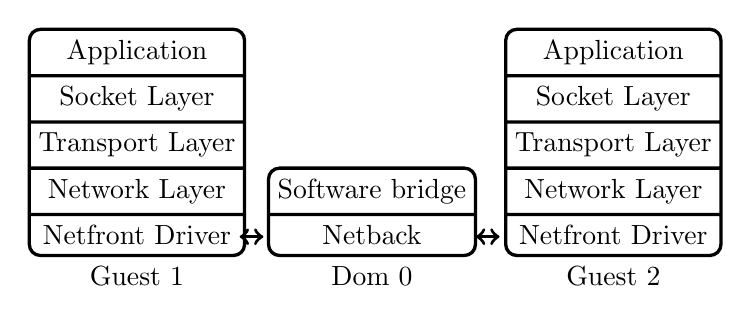
\begin{tikzpicture}
      [domU/.style={
           rectangle split,
           rectangle split parts=5,
           rounded corners,
           draw=black, very thick,
           text centered,
           anchor=five
         },
       dom0/.style={
           rectangle split,
           rectangle split parts=2,
           rounded corners,
           draw=black, very thick,
           text centered,
           anchor=two
         },
       ]
    \node [domU, label=below:Guest 1] (dom1) at (-3,0) {
      Application
      \nodepart{two}
      Socket Layer
      \nodepart{three}
      Transport Layer
      \nodepart{four}
      Network Layer
      \nodepart{five}
      Netfront Driver
    };
    
    \node [domU, label=below:Guest 2] (dom2) at (3.05,0) {
      Application
      \nodepart{two}
      Socket Layer
      \nodepart{three}
      Transport Layer
      \nodepart{four}
      Network Layer
      \nodepart{five}
      Netfront Driver
    };

    \node [dom0, label=below:Dom 0] (dom0) at (0.55,0) {
      Software bridge
      \nodepart{two}
      Netback
    };

    \path (-0.5,0.1) edge [draw=black, very thick, <->] (-0.2,0.1);
    \path (2.5,0.1) edge [draw=black, very thick, <->] (2.8,0.1);
    
  \end{tikzpicture}
  \caption{Normal IP architecture of Xen domUs}
  \label{xen_normal_architecture}
\end{figure}


Xen offers a way to directly share memory between hosts.
Using such dedicated memory should allow to create channels between virtual hosts with only a few data copies and little to no kernel involvement.

\subsection{Related work}

The Xen's \emph{grant table} feature offers an interface for different \emph{domU} kernels to share memory pages with each other, allowing different domain's drivers to share information and making optimized communication channels possible. As the perspective of obtaining a very fast communication system appeared to be very attractive, some solutions has been proposed. XenSocket\cite{XenSocket} provides the user a new socket interface (\emph{AF\_XEN}), so that only a few modifications are needed at the application layer. XWay\cite{XWay} implements a new transport layer, under the \emph{INET} layer and over the \emph{TCP} layer, and use a shared memory channel whenever it is possible, so that no modifications are needed at the application layer. XenLoop\cite{XenLoop}, finally, acts at the IP layer, offering the advantage of not only being fully transparent but also supporting migrations. 

As the Xen's \emph{grant table} interface changes a lot, most of those implementations would need modifications in order to compile (they are not maintained). Actually, the only well maintained driver we found is \emph{gntdev}. It enables shared memory mapping into the user space, but doesn't provide any communication interface. 
We didn't chose to not use this device, but its source code helped us in achieving mapping of shared memory into the user space. 

\subsection{Our work}

Those solutions are pretty efficient and very user friendly, letting no much more space for improvement, but all of them, as the user space cannot directly access the shared memory, require system calls (and thus context switching) in order to achieve read and write operations.
They are, therefore, less efficient than it could theoretically be. 
In this report, we present our own optimized communication system, based on shared memory. It performs way better than other existing solutions but, as a trade-off, needs the user to be aware of some particularities.

\begin{figure}[h]
  \centering
  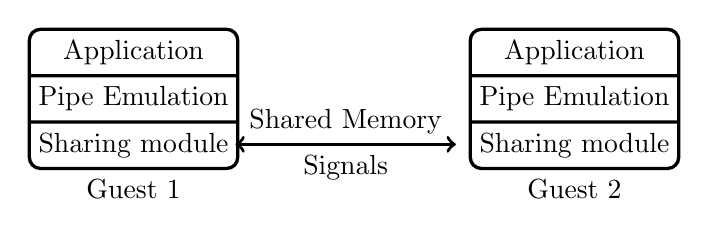
\begin{tikzpicture}
      [domU/.style={
           rectangle split,
           rectangle split parts=3,
           rounded corners,
           draw=black, very thick,
           text centered,
           anchor=three
         },
       ]
    \node [domU, label=below:Guest 1] (dom1) at (-2.8,0) {
      Application
      \nodepart{two}
      Pipe Emulation
      \nodepart{three}
      Sharing module
    };
    
    \node [domU, label=below:Guest 2] (dom2) at (2.8,0) {
      Application
      \nodepart{two}
      Pipe Emulation
      \nodepart{three}
      Sharing module
    };

    \path (-0.3,0.1) edge [draw=black, very thick, <->] node [above] {Shared Memory} node [below] {Signals} (2.5,0.1);
    
  \end{tikzpicture}
  \caption{Optimised channel using shared memory and signals}
  \label{xen_shm}
\end{figure}


Our implementation is divided into two parts. First, the Xen shared memory tool, a device kernel module, provides a way of sharing memory between two user-spaces of possibly different virtual machines on the same Xen hypervisor. For performances purposes and because of possible dead-locks, it also uses a bidirectional event channel and therefore provides the user \emph{wait} and \emph{notify} operations.

The second layer of our solution, a user space library on top of the kernel shared memory module, provides a \emph{file-like} interface, allowing the user to set-up a unidirectional channel and use it to send or receive data. It abstracts the inner work that transforms memory into an optimized circular buffer that only makes necessary system calls.

In the second and third parts of this report, we detail the functioning of those two different elements. Then, in the fourth part, we present the performances of our solution. 

\section{Shared memory device}

The first realisation of our project is a Linux kernel module which defines a new device driver\footnote{Its current name is xen\_shm}.
According to the end-to-end principle, it's a really dumb module that just gives the user tools to share memory, signals and detect disconnection, without any practical protocol for how to use it.
As the Linux kernel, and more precisely its Xen parts, always change, our module is only guaranteed to work on Linux kernel version 3.2.32 (Debian testing), 3.4.9 and 3.5.4 (Gentoo Linux stable).

\subsection{Xen shared memory}
\label{xen_shared_memory}

In the normal Xen model, each virtual host have its own memory address space which are mapped to non-overlapping physical memory, providing the usual abstraction of total ownership of the memory space to each host. Nevertheless, the Xen hypervisor can also remap some host's memory into the address space of another host. In order to do so, an host $A$ must ask the hypervisor to grant the right to use a given part of its physical memory to a given host $B$. The hypervisor will issue a ticket, called grant reference, which can be used by $B$ to map the physical memory from $A$ into its own address space.

The implementation of this protocol can be considered as a potential security breach: from our experiments, we tend to believe that the entropy of the domain id (16 bits) and the ticket (32 bits) is really small (and the tickets seems to be simply increasing). Thus an attacker that obtained access to one of the two hosts, as long as it have access to the userspace tools to map the memory, could also, by guessing or brute-forcing those ids, map the same physical memory and thus spy or modify the data. Such a security problem doesn't come from our system but from Xen, thus we believe that it will be fixed in the near future.

Another restriction of this model concerns hot migration of hosts. If a group of hosts shares two-by-two some memory then none of them can be migrated to another machine as it is not possible to share physical memory between two distant nodes (at least with the current technology). The current sharing mechanism and grant system doesn't provide a way to detect and prevent or cope with such migrations, thus our system will probably utterly crash if this occurs. If such an API is provided by Xen in the future, mechanisms that disable the channel could be implemented.

\subsection{Create shared memory}

In order to share some memory, the memory first needs to be allocated in one of the two hosts, that we will call the \emph{offerer}\footnote{This will have implications for the clean termination and memory freeing, as explained later, see section \ref{Termination}.}. When an host do so, it allocates different things, some pages in the real\footnote{In that case, what he believes real, which is protected by Xen.} physical memory and some address space that will be mapped to it. As grants are given on an host to host basis, the \emph{offerer} needs to know the domain id of the other host which will be called the \emph{receiver}. The exact specification of such exchanges of information, using standard communication paths, is outside the scope of our project\footnote{Reader are invited to look at the simple protocol using UDP that we created for that purpose during our test}. Then, by using an \emph{Hypercall}, the \emph{offerer} can ask the hypervisor to grant the right to map. The hypervisor will store the pseudo-physical address that corresponds to the grant, together with the domain id of both the \emph{offerer} and the \emph{receiver} and also a ticket number.

With both the \emph{offerer's} domain id and the grant ticket number, the \emph{receiver} can make another \emph{Hypercall} with some references of its own address space: the hypervisor will take care of modifying the memory mapping between the two spaces. Mapping in the kernel space is easy, as we fully control what happens. Mapping in the user space, a separate domain with a lot of automatic events, is harder as we will explain in the next section. 

In fact, we are not using directly the Hypercalls. Those are pretty stable but needs work to be done around them depending on the hardware, the kernel/Xen versions and so on. Recent Linux kernels provide an API to abstract all of this, but this API have recurrent small changes\footnote{For example the function \emph{gnttab\_unmap\_refs} is different between the three kernel we used.} as more functionalities are added. Even if this API is currently more volatile, we still believe that using it will provide a better long-term stability.

\subsection{Initialization}

When a user opens the device, private variables are initialized, but no hypercalls are made, so that the instance could equally become an \emph{offerer} or a \emph{receiver}. To configure the instance, particular \emph{ioctl} operations must be used\footnote{For more information, the source code headers are appropriately commented}. Some of them return values such as the local domain id or the grant reference (ticket). 
Those values then need to be shared so that the other process can call appropriate \emph{ioctls} and configure the instance on its own side. 

In our implementation, each shared page uses its own grant reference (ticket). In order to reduce the size of the information that needs to be shared, the first page is used as an header page. This page contains all the needed grant references, event channel information, and the state of both ends (they are correctly maintained as long as no kernel crashes). Therefore, the first page the user can map is only the second shared page. 

\subsection{Map memory into user-space}
\label{userspace}

As this implementation tries to limit the kernel involvement, it maps directly the shared memory into the userspace, allowing direct read/write accesses without any overhead.

On the \emph{offerer} side, the mapping is easy as the kernel already prepare all the work for device drivers: when standard device driver functions are called (open, nmap, munmap, close), the kernel automatically prepare or clean the memory. Furthermore, a function, \emph{remap\_pfn\_range}, exists for simple remapping, making this remapping a child problem.

On the other side, the \emph{receiver} one, things are more complicated. At first sight, one can simply call the xen API with the user space address. It will somehow work, that is it will map the physical memory and grant the access as we want, but it won't last long as it will taint the kernel with page errors during the unmapping.
The correct approach is to work on a lower lever, page tables, and to correctly invalidate the mapping on an early stage of the memory unmapping\footnote{Dedicated MMU Notifier Operation are registered in the memory management system in order to do so.}.
This part of our work is inspired by the Linux \emph{gntdev} driver that allows to map memory into user space (But without all the automatic exchanges nor the signals that we wanted). Even if our code was fully rewritten for simplicity purposes, maintainers and users are encouraged to monitor modifications of this part of the Kernel on each major update as it will be probably be maintained by Linux kernel or Xen developers as new functionalities kicks in.

\subsection{Event channel}

Shared memory is essential to provide any communication system, but when it comes to make it more efficient, it is not enough anymore. Indeed, when there is no data available, the \emph{reader} must wait for it. Also, when there is no more space, the \emph{writer} has to wait too. On a single host, the kernel is usually responsible of making the processes wait and wake them up when needed. Also, \emph{mutexes} are used in user space in order to synchronize different processes. But those solutions simply doesn't work when different kernels are using shared objects.

Therefore our device, in addition to shared memory, uses an event channel in order to provide \emph{wait} and \emph{notify} operations. An event channel is a bidirectional pipe able to send and handle virtual interrupts, through Xen's hypercalls. Creating an event channel is very similar to sharing memory. The \emph{offerer} opens an event channel, identified by its port number, while the \emph{receiver} uses the port number with the distant domain id in order to connect to it.
When the \emph{offerer} process initializes its own side, the port number is written in the header shared page so that it can be read by the \emph{receiver} and the channel established. 

Even though an event channel only transmit one bit of information, the user space interface, using \emph{ioctls}, provides different features. Indeed, upon connection of the event channel, a very first signal is sent to notify the \emph{receiver} that some process successfully connected to the other end. This signal is acknowledged so that both ends know that the other process is ready. This mechanism allows the user to wait for initialization, which should be used instead of the \emph{accept} call of TCP sockets.

Then, there exists two different way to wait for other user's signals. The first and most obvious consists in waiting for a signal which is received while the process is waiting. Which means that the process will only be waken up by the kernel if some received signal is handled after the kernel put the process in the waiting queue.  But this way to wait, because of possible race conditions, can be unsafe. Therefore, the user process can also wait for a signal that could have been received before the process was put in the queue, but which did not woke up any process. The triggering signal could be outdated, but this feature prevents possible deadlocks. 

Those three different kind of signals can be used together with two other features. The first is a very classic \emph{timeout} feature, which allows the process to wake-up after some time\footnote{Specified in ms but only performs with jiffies precision} if no signal have been received. The second feature consists in returning immediately if the other process is already waiting. It uses atomic operations on a shared integer, but its correctness only relies on kernel's and hardware's atomic operations correctness. Therefore, although it significantly reduces the probability of a deadlock to happen, we preferred not to use it in the pipe implementation, privileging higher layer solutions.

\subsection{Termination}
\label{Termination}

Outside the correct memory invalidation that we talked about in section \ref{userspace}, because of the non-symmetrical model of the memory sharing, special care is needed before completely cleaning the module. The initial physical space belongs to the \emph{offerer}, that internally allocated it, mapped it and told Xen about its exact location. When closing the module, the \emph{offerer} needs to free it as we don't want such enormous memory leakages. But as we are talking about direct mapping, if the \emph{receiver} still have an active mapping, it will be able to modify the physical memory.
If the \emph{offerer} frees the memory without any check, it will be potentially re-allocated later somewhere else by any application or kernel actions and if the \emph{receiver} modifies it at this point, unspecified errors are expected from the resulting non-desired sharing.

The Xen API provides methods to detect the number of active mappings per grant. As a result our implementation checks for potential active mapping and prevents memory freeing if necessary. From the user point of view, the mapping will be undone and the function call returns immediately but internally information about memory is kept and the unmapping is scheduled to take place later.

Both sides kernels also maintained a shared state field, inside the header page, which indicates whether the end user is using the opened instance or not. Those fields are monitored so that any waiting process immediately returns with \emph{EPIPE} error if the other end state becomes closed. As the kernel monitors and close files when some process crashes, this ensures broken pipe detection as long as no kernel panic occurs.

\subsection{Security considerations}

In section \ref{xen_shared_memory}, we stated the possibility for a third party, on the receiver's domain, to access the shared memory by brute forcing the domain id and the grant reference. This design flow weakens our protocol's security, but also Xen's security itself. Indeed, as both grant reference and domain id suffer from a serious lack of entropy, it becomes possible for two virtual machines to establish a communication channel, even though the \emph{dom0} forbids them any form of communication. For instance, if an attacker could access \emph{/dev/gntdev}, it could use it to transfer data to another domain owned by the attacker, bypassing all IP protections. 

Xen's administrators should be aware of this flows. But as this grant table feature is not fully mature\footnote{Recurrent modifications of the Linux API}, we hope that Xen's developers will fix that missing entropy and perhaps implement a better access control on grant tables like, for example, a system where dom0 would be able to white list couples of domains that can share memory between them.

\section{Shared memory based circular buffer}

Once two processes share memory, they can obviously transfer data, but our goal in this project was to offer an optimized pipe, as fast as it possibly can, while remaining resource efficient. Therefore, the pipe library not only offers a more user-friendly interface for transmitting data using the shared memory device, but it also implements different optimization techniques that provide much better performances than any other state-of-the-art solutions. 

\subsection{Principles}

The unidirectional communication channel relies on the very simple and well known circular buffer structure, which offers the pretty interesting particularity that it is wait free as long as it is neither empty nor full. The \emph{writer} and the \emph{reader} share their own position cursor, indicating where they currently are and how far the other peer can go in the buffer. Both peer also keep a flag field that allows them to gives some more information about their state. A flag, for example, is used to close the pipe. Typically, the \emph{writer} sets it when he has nothing left to writer, just before closing the device. 

Although we cannot be as transparent as existing solutions, our implementation was conceived to be as user friendly as possible. The bootstrap needs the peers to exchange information and to call different functions, but once it is done, the interface is very similar to the file interface. 

As it is a unidirectional channel, peers are called \emph{writer} and \emph{reader}. One pipe, using some shared memory instance, needs exactly one \emph{writer} and one \emph{reader}, but those roles have nothing to do with the underlying \emph{offerer} and \emph{referer} roles, which refer to the owner of the physical memory. Some peer can be whether the \emph{offerer} or the \emph{receiver}, as long as they use the same convention. Nevertheless, note that it is best practice to make the \emph{reader} to be the \emph{offerer}. Indeed, during a graceful transfer, the \emph{writer} usually decides when we wants to stop transmitting, and it is better to close the \emph{receiver} before the \emph{offerer} so that every shared entry can be immediately ungranted (otherwise it has to be put in the 'close later' queue).

\subsection{Optimizations}

Circular buffers are very simple structures, but optimizing them can be tricky. The first, and obvious, optimization consists in copying words instead of bytes. As our evaluation systems use 64bits processors, we optimized the copying to be done on 64bits aligned words. Therefore, it is best-practice to use 64bits aligned buffers when performing read and write operations. 

When the buffer is full (resp. empty), the writer (resp. the reader), must wait. Also, when data or space becomes available, some process must notify the other process. But those two operations can only be performed through system calls. That's why we also needed to reduce the number of \emph{wait} and \emph{notify} calls. 

First, to reduce the number of \emph{notify} calls, the \emph{sleeping} flag is used to tell whether a process is waiting or not. A process checks this flag at least one time per \emph{read} or \emph{write} call, and four time per buffer round (so a process is only woke up when there is a significant amount of available data/space), and sends a signal if necessary (if the \emph{sleeping} flag of the other peer is set).
On the other hand, a process sets this flag just before calling the \emph{wait ioctl}, and unsets it after wake up. Of course, this creates a race condition, but we explain how this problem was solved in the next section.

Then, we also want to avoid unnecessary \emph{wait} calls. An obvious way to do it would be to loop until data/space is available, and it would work, as long as the process is alone on the machine. Otherwise, the kernel scheduler would unschedule the process, which would significantly reduce the performances. Moreover, it wouldn't be resources efficient.
As a solution, we use the \emph{active} flag in order to tell the other process whether we are currently doing something or not.
If set, the other process will wait actively (loop) instead of calling the \emph{wait} ioctl (and so the other process will not call \emph{notify}). Nevertheless, when a lot of processes are running, a process can be unscheduled, and the other process can loop for nothing. Therefore, there is a limitation to the number of consecutive loops after which the process will try to sleep. This limit is empirical and the optimal value depends on the number of processes. A large value is optimized for a few processes running at the same time while a smaller value will allows the channel to bear more frequent unscheduling.  

\subsection{Dead-lock avoidance}

Of course, a process must be extremely careful before putting itself into sleep, or even while looping, because the other process could whether be waiting, or even crashed. That's why we use another flag, \emph{waiting}, that a process sets whenever we starts waiting for data/space\footnote{The wait can be active (looping) or passive (sleeping)}, and unsets it at the end. The key idea, of course, is to forbid sleeping when the other process set this flag\footnote{An important point for efficiency is to notice that there is whether space or data available, so even if both processes can wait at the same time, it can't be the case for very long}, which implies a weak form of consensus.
Using only registers, this cannot be solved by a deterministic algorithm, but as both processes should never wait at the same time, we found a way to solve the problem. The basic idea is to continue looping as long as there is no available data/space. At the beginning of each loop, we set the waiting flag, and then see if the looping condition is still true.
This ensures that the other process could not have entered the waiting loop before we set the flag. And therefore, he knows we are waiting, which prevents him from sleeping.

As we said earlier, a process doesn't always sends a signal after an operation, even though the other process is going to wait for it (there is a race condition). This is not a problem as long as both processes continue writing and reading, because everything is done to wake up sleeping processes. But, if some process wants do to something else, nothing ensures the other process will be able to full/empty the buffer completely. Therefore, we provide the user the \emph{flush} function, which will simply sends a signal through the event channel. Because of the way we wait for signals\footnote{A signal, if not immediately handled, wakes up any future waiting process}, sending such a signal ensures all the data/space that was available before the user called \emph{flush} to be correctly handled by the other process. 

\subsection{Closing the pipe}

Whenever a process closes the pipe, it sets the closed flag, so that the other peer can know it. When it's set, any \emph{write} will fail and \emph{read} will return end of file as soon as there is no more available data.  

But we still have a problem if some process crashes. When it occurs, the kernel will close the device file, modify the shared state, and send a signal, so that any waiting process will receive the \emph{EPIPE} error. But in some previously described cases, a process is prevented from sleeping (active loop). So each process that makes more than a fixed number loop must check if the channel is still open. It is done by waiting for the initialization signal, so that it whether returns 0 or \emph{EPIPE}. 

Those mechanisms, put together, offer graceful termination and prevent dead-locks. Nevertheless, processes can loop when the other kernel crashes. The event channel could be used to send regular keep-alive, but we did not have the time to implement it.  

\section{Evaluation}

Because of the instability of the Xen system and of the Linux kernel, it is currently not possible to do an exact comparison between other similar idea/implementation. In order to be as fair as possible we chose to use old hardware that dates from approximately the same period as the quoted related work.

\subsection{Configuration}

Our experiments were run on an Intel\textregistered ~Core\texttrademark 2 Quad Processor Q9550, running at 2.83 GHz with a L2 cache of 12MB and equipped with 4GB of standard DDR2-800 RAM. We are aware that such a system is not representative of recent dedicated virtualization servers, but results are still impressive.
With the recent improvements of caches, sharing mechanisms inside CPUs and memory access, we believe that our system will present far better results on modern systems. For example, tests run inside a virtualized environment on a two years old Intel\textregistered ~i7 processor showed result close to an order of magnitude better that the ones presented in this report, but fairness with other existing implementation was, we think, more important.

The final tests were run using Xen 4.2.1 on top of Linux 3.5.7. We used the Gentoo Linux distribution for both the dom0 and the domUs. We also pinned the CPUs: dom0 always had 2 CPUs and 2GB of memory. Depending on the tests, either we used two hosts with 1 CPU and 1GB of memory each, either we used only one other host with 2 CPUs and still 1GB of memory. We allocated a lot of memory to each hosts but almost none of it was used by our system that only allocate one shared buffer.

\subsection{Throughput}
\label{section:throughput}



The first thing we tested was the throughput, as shown in figure \ref{shm_size}. We used \emph{iperf} to evaluate the domU to domU throughput for a fixed packet size but different window size, then we compared to our solution, using the same amount of memory that was used for the tcp window for our shared memory. As expected we outperform the tcp throughput by a factor of at least 5.

\begin{figure}[h]
\centering
\begin{tikzpicture}
    \begin{semilogxaxis}[
        xlabel=Buffer size (KiB),
        ylabel=Throughput (Gbps),
        legend style={nodes=right},
        legend pos= north west,
        scaled ticks=false, 
        compat=1.3
        ]
        
    \addplot table [ x index=0,y index=1] {plots/bandwidth.txt};
    \addlegendentry{Xen pipe}
    
    \addplot table[ x index=0,y index=3] {plots/bandwidth.txt};
    \addlegendentry{Stressed Xen pipe}
    
    \addplot table[ x index=0,y index=2] {plots/bandwidth.txt};
    \addlegendentry{TCP}
    
    
    \end{semilogxaxis}
\end{tikzpicture}
\caption{Comparison between Xen pipe and TCP throughputs for different buffer sizes}
\label{shm_size}
\end{figure}


As no other process were running at the same time, the test was a bit unfair: as the processor cache was not used by anyone else, the shared memory was fully contained in it and it was never invalidated by some concurrent process\footnote{We only used 2 processes as the domain add 2 CPUs, in order to have no scheduling concurrence.}. In order to be fair, we made the same test under some pressure. An other process was writing as fast as it can into an address space larger than the buffer size, thus invalidating as fast as possible all cache entries. The result are interesting: when you use only a few pages, the other process has only a small impact. We think it's because the probability of having our few pages invalidated among all the cache entries is small. Then, when you add more pages, at some point you loose throughput, also probably because you increase the collision probability.

\begin{figure}[h]
\centering
\begin{tikzpicture}
    \begin{semilogxaxis}[
        xlabel=Message size (Bytes),
        ylabel=Throughput (Gbps),
        legend style={nodes=right},
        legend pos= north west,
        scaled ticks=false, 
        compat=1.3
        ]
        
        
        \addplot table[x index=0,y index=4] {plots/messageSize.txt};
    \addlegendentry{XenPipe: 60}
        
      \addplot table[ x index=0,y index=3] {plots/messageSize.txt};
    \addlegendentry{XenPipe: 20}  
        
        
     \addplot table[  x index=0,y index=2] {plots/messageSize.txt};
    \addlegendentry{XenPipe: 5}   
        
    \addplot table[  x index=0,y index=1] {plots/messageSize.txt};
    \addlegendentry{XenPipe: 1}
    
    
    \addplot [smooth,dashed,mark=*,orange] table[  x index=0,y index=5] {plots/messageSize.txt};
    \addlegendentry{XWay}
    
    \addplot [smooth,dashed,mark=square*, violet]  table[  x index=0,y index=7,orange] {plots/messageSize.txt};
    \addlegendentry{XenSocket}

    \addplot [smooth,dashed,mark=x, magenta] table[  x index=0,y index=6] {plots/messageSize.txt};
    \addlegendentry{XenLoop}
   
    \end{semilogxaxis}
\end{tikzpicture}
\caption{Throughput of Xen Pipe with different shared memory sizes (indicated in pages) and other state-of-the-art solutions with respect to the message size}
\label{msg_size}
\end{figure}


Then we compared different message size and different shared memory size as shown in figure \ref{msg_size}. For small message size, as long as the shared memory size is bigger than the message size, performances are the same, but as soon as messages cannot fit in one piece in the memory the throughput is degraded. We currently have no explanation for the irregularity that present the curve with 60 pages and this over-performance need to be studied more. This figure also include curves for other existing solutions. As we weren't able to compile and run them, the numbers come from their original papers. It is clear that our optimization improved the performances.

\subsection{Delays}

Another area where our solution is supposed to increase the performances is the delay between the emission and the reception between the two VMs. For the references, we used two domains, each with there own CPU and let them exchange ICMP query/reply. The mean of the Round Trip Time (RTT) was about $114 \mu s$. An interesting point here was that the very first first ICMP exchange (of series) always took more than three times the mean (We excluded it from the mean calculus). It tends to indicate that even ICMP need to take time to initialize itself, thus, even if we didn't measured the initialization time of our solution (exchanging information and sharing memory), should not be that worse than standard TCP handshakes (plus the time needed to initiate the routes as even ICMP need time to do so).

We did two different kind of measurements that tries to reproduce pings, a \emph{ping} flood and isolated \emph{pings}. In both cases, after the initialization, one host writes in one pipe a predetermined amount of data (small as we don't want bandwidth to have an impact), the other reads in the same pipe the same fix amount and write it back in an other pipe that is read by the first host. This simple system allows up to measure the time needed to exchange information, a virtual RTT. The results outperform ICMP exchanges: in isolated pings, the RTT was about $41 \mu s$ and in ping flood it was down to $24 \mu s$, less than a fourth of ICMP one !

It is clear that in the case of the ping flood, it is our optimization that reduce the number of wait that allows such good performances, which means that we have an interesting trade-off between response time and length of active wait. In the case of the isolated pings, even if the process is waiting and an interrupts is used to notify it, we are still twice faster than the IP-based solution.

\subsection{Simultaneous transfers}

As we saw in section \ref{section:throughput}, our performances probably depends on the utilization of the cache by other programs or threads. An interesting comparison is then the impact of simultaneous transfers: do they disturb each other or not ? In order to check this question, we fixed two CPUs on dom0 and two CPUs on a domU and measured the throughput of processes flooding their channel, varying the number of processes in each measurement. The aggregated results are shown in figure \ref{simult_flows}.



\begin{figure}[h]
\centering
\begin{tikzpicture}
    \begin{semilogyaxis}[
        xlabel=Number of parallel flows,
        ylabel=Throughput (Mbps),
        legend style={nodes=right},
        legend pos= south west,
        scaled ticks=false, 
        y tick label style={/pgf/number format/.cd,sci,precision=5},
        compat=1.3,
        ]
        
        
        \addplot [blue,mark=x] table[x index=0,y index=1] {plots/multi.txt};
    \addlegendentry{Total throughput}
        
     
    
    \addplot [smooth, red] table[x index=0,y index=8] {plots/multi.txt};
    \addlegendentry{Optimal sharing}
    
     %\addplot [smooth, black] table[x index=0,y index=5] {multi.txt};
    %\addlegendentry{Median value}
    
    %\addplot [smooth, gray] table[x index=0,y index=6] {multi.txt};
    
    %\addplot [smooth, gray] table[x index=0,y index=7] {multi.txt};
       
    %\addplot [smooth, lightgray] table[x index=0,y index=3] {multi.txt};
    
    %\addplot [smooth, lightgray] table[x index=0,y index=4] {multi.txt};
    
    \addplot [box plot median] table {plots/boxes.txt};
    \addplot [box plot box] table {plots/boxes.txt};
    \addplot [box plot top whisker] table {plots/boxes.txt};
    \addplot [box plot bottom whisker] table {plots/boxes.txt};
    \addlegendentry{Values distribution}

    
    \end{semilogyaxis}
\end{tikzpicture}
\caption{Throughputs of multiple parallel flows (60 shared pages per transfert - messages of 32KiB - average value over more than 20 seconds). The dark line corresponds to the median value. 
Gray lines correspond to first and last decile. Light gray lines correspond to the maximum and minimum values}
\label{simult_flows}
\end{figure}


For up to 10 processes, the sharing is perfect and, in some cases achieve more global throughput that the one process case. For bigger numbers of processes, the sharing is less good than before with more dispersion and lower total throughput, even if the total throughput only decrease by a factor of two to three in the worse case. We think that in that case the major problem was the scheduling on two cores of a high number of concurrent processes creating a lot of context switching. It is possible that by changing the length of our active wait we could have achieved better total throughput with less dispersion, but we didn't have the time to do a full analysis.

\section{Conclusion}

\subsection{Contributions}

In this report, we presented Xen Pipe, an optimized communication channel that uses Xen's memory sharing mechanisms. In contrast to the existing solutions, it moves most of the operations at the user level and thus approaches optimal throughputs (limited by memory speed). Our work was divided into two main parts.

The first contribution consists in the shared memory device, which offers a way to share memory between two \emph{user} processes on possibly different domains, and implements connection-aware features. It is not only the first time a kernel device driver joins those two features but, because of the evolution of Xen's interface, our source code can be used as a reference for memory granting and mapping for recent Xen's versions.

As a second contribution, our work focused on the way shared memory can be used as an optimized channel medium, focusing on the idea that only a few system calls are absolutely necessary when transmitting data. Different optimization ideas were introduced and the results are impressive. While resources efficient, our solution offers better throughput than any other existing solutions. As a trade-off, the user must be aware of some peculiarities, but future work could offers a more user friendly API, needing only a few modifications at the application layer.

\subsection{Possible improvements}

Although our solution is running, it is quite far from ready for production. First of all, it can only run on a few kernel and Xen versions, the use of shared structures could induce serious endianness problems, and a deeper debugging should be done. Also in a more practical point of view, we see at least three axes of possible improvements.

First, we didn't implement any security mechanisms. The memory sharing mechanisms should prevent multiple domains to map the same shared area. This could be done, for instance, by ungranting the memory area access as soon as the initialization signal is received, ensuring that only one mapping is done, and finally identifying the receiver. Doing so, no third process could interfere, and no man-in-the-middle attack would be possible as long as the bootstrapping mechanism is secured. 

As a second future work axe, we think the unscheduling detection could be improved. Indeed, by now, when a process is unscheduled while writing or reading data, the other process loops a certain constant number of iterations, waiting for data or space, before assuming the other process was unscheduled, and then, go to sleep. The ideal number of iterations depends on processors speed and the regularity with which cursors are moved by peers (they are moved by steps, not continuously). Those steps should be variable and depend on the regularity of detected unscheduling. The idea is to approach unscheduling detection as TCP adapts to packet losses. 

Finally, as a third point of improvement, the API would need some revisions. First, the transfer convention (writer offerer or writer receiver) and mod (write or read) shouldn't have to be specified at the initialization of a pipe. Indeed, it reduces the possibility of agreements that could be made by the upper IP protocol. Then, a bootstrap mechanism should be developed in order to provide a bidirectional pipe by only providing a file descriptor (typically a TCP connection between the two hosts). Ideally, a mechanism should allow the peers to know if they are on the same physical machine or not.

\begin{thebibliography}{1}

\bibitem{XenSocket}
Xiaolan Zhang et al., \emph{XenSocket: A High-Throughput Interdomain Transport for Virtual Machines}, Middleware '07.

\bibitem{XWay}
Kangho Kim et al., \emph{Inter-domain Socket Communications Supporting High Performance and Full Binary Compatibility on Xen}, VEE '08.

\bibitem{XenLoop}
Jian Wang et al., \emph{XenLoop : A Transparent High Performance Inter-VM Network Loopback}, HPDC '08.

\bibitem{gntdev}
Derek G. Murray, Grzegorz Milos and Steven Hand, \emph{Improving Xen Security through Disaggregation}, VEE '08.

\end{thebibliography}

% that's all folks
\end{document}


